\documentclass[12pt]{jreport}
\usepackage{comment}
\usepackage{./sty/eclepsf}
\usepackage{tascmac}
\usepackage{tabularx}
\usepackage{listliketab}
\usepackage[longnamesfirst]{natbib}
\usepackage[dvipdfmx]{graphics}
\usepackage[dvipdfmx]{graphicx}
\usepackage[dvipdfmx]{color}
\usepackage{subfigure}
\usepackage{alltt}
\usepackage{here}
\usepackage{afterpage}
\usepackage{./sty/ncodeline}
%\usepackage[dvipdfmx, colorlinks, breaklinks,%
\usepackage[dvipdfmx, breaklinks,%
bookmarks=true, bookmarksnumbered=true,%
bookmarkstype=toc, bookmarksopen=true,bookmarksopenlevel=3,%
pdftitle={RG},%
]{hyperref}
\usepackage{bookmark}

\AtBeginDvi{\special{pdf:tounicode EUC-UCS2}}

\usepackage{diagbox}

\usepackage{fancyhdr}

\usepackage{./sty/doxygenorig}

\usepackage{indentfirst}
\usepackage{url}
\usepackage{listings,./sty/jlisting}

\def\lstlistingname{プログラム}

\lstset{%
 language={C++},
 %backgroundcolor={\color[gray]{.85}},%
 basicstyle={\small\ttfamily},%
 identifierstyle={\small},%
 commentstyle={\small\itshape},%
 keywordstyle={\small\bfseries},%
 ndkeywordstyle={\small\ttfamily},%
 stringstyle={\small\ttfamily},
 frame={tb},
 framesep=1zw,
 breaklines=true,
 numbers=left,%
 xrightmargin=0zw,%
 xleftmargin=1.5zw,%
 numberstyle={\scriptsize},%
 stepnumber=1,
 numbersep=1zw,%
 lineskip=-0.5ex%
}

\usepackage{amssymb}
%\usepackage{supertabular,multirow}

\usepackage{array}
\newcolumntype{M}[1]{>{\centering\arraybackslash}m{#1}}

% A4  size: 297mm*210mm %1pt = 0.35mm
\setlength{\topmargin}{-3.4mm} % 10pt 25.4mm - 3.4mm = 22mm
\setlength{\oddsidemargin}{-0.4mm} % 25.4mm - 0.4mm = 25mm
\setlength{\evensidemargin}{-0.4mm} % 25.4mm - 0.4mm = 25mm
\setlength{\textheight}{231mm} % 660pt % original is 225.75mm 645pt
\setlength{\textwidth}{160mm} % 457pt

\renewcommand{\topfraction}{.99}
\renewcommand{\textfraction}{.0}
\renewcommand{\floatpagefraction}{.99}
\renewcommand{\bibname}{参考文献}


\pagestyle{fancy}
\lhead[]{}

\makeatletter
\def\chaptermark#1{\markboth {\ifnum \c@secnumdepth>\m@ne
\@chapapp\ \thechapter \@chappos\ \fi #1}{}}
\makeatother

% タイトル
\def\title{ソーシャルメディア上の噂により買いだめ行動が起きる現象への


感染症モデルの応用}
% 英語タイトル
\def\etitle{English Title}
% 著者(日本語)
\def\author{後藤 悠太}
% 著者(英語)
\def\eauthor{Yuta Goto}
% 学部・研究科
\def\dept{慶應義塾大学 環境情報学部}
% 学部・研究科(英語)
\def\edept{Keio University Faculty of Environment and Information Studies}

\begin{document}

\pagenumbering{roman}
\begin{titlepage}
  \begin{center}
    \begin{large}
      卒業論文   2020年度(令和2年)\\
      \vspace{24pt}
      \title
      \end{large}
  \end{center}
  \vspace{40em}
  \begin{flushright}
    \large \dept\\
    \author
  \end{flushright}
\end{titlepage}

\thispagestyle{empty}


卒業論文要旨 - 2020年度 (令和2年度)
\begin{center}
\begin{large}
\begin{tabular}{|M{0.97\linewidth}|}
    \hline
      \title \\
    \hline
\end{tabular}
\end{large}
\end{center}

~ \\

趣旨を記載する

~ \\
キーワード:\\
\underline{1. 予言の自己成就},
\underline{2. トイレットペーパー買いだめ},
\underline{3. aaa},
\underline{4. bbb}
\begin{flushright}
\dept \\
\author
\end{flushright}

\thispagestyle{plain}
\clearpage

Abstract of Bachelor's Thesis - Academic Year 2020
\begin{center}
\begin{large}
\begin{tabular}{|p{0.97\linewidth}|}
    \hline
      \etitle \\
    \hline
\end{tabular}
\end{large}
\end{center}

~ \\

Describe the purpose of this research.

~ \\
Keywords : \\
\underline{1. self-fulfilling prophecy},
\underline{2. hoarding},
\underline{3. aaa},
\underline{4. bbb}
\begin{flushright}
\edept \\
\eauthor
\end{flushright}

\thispagestyle{plain}
\clearpage

\tableofcontents\thispagestyle{plain} %目次
\clearpage
\listoffigures\thispagestyle{plain} %図目次
\clearpage
\listoftables\thispagestyle{plain} %表目次
\clearpage

\pagenumbering{arabic}
\chapter{序論}
\label{introduction}

本章では本研究の動機,課題及び手法を提示し,本研究の概要を示す.

\section{はじめに}
\label{introduction:background}

ソーシャルメディア上の根拠のない噂が、現実となることが実社会で起きている。
これは、個人の合理的な利益追求行動が集団に不利益をもたらし、結果として個人にとっても悪い結果をもたらす社会的ジレンマと考えられる。
また、こうした現象は「予言の自己成就」として、人々が社会現象についての予言(予測)を信じて誤った認識をいだいて行動するために、結果的にその予言が実現する現象を指すとされてきた。
アメリカの社会学者R.K.マートンは、予言の自己成就に対して、最初の誤った状況の規定によって新たな行動が発生して、その行動が最初の誤った行動の規定を現実のものとしてしまうことであるとしている。\\*
 
具体的な事例として、銀行の取り付け騒ぎ~\cite{}がある。
支払いが不可能になるとの噂が発端となり、預金の引き出しが殺到して、結果として噂の通り支払いが不可能な状況を作り出してしまうというものである。
また、国家間における軍拡や戦争の事例も同様である。
対立関係にある2国間では、相手側の攻撃的な発言や動きに対して不安が強まり、結果として軍拡が進められ、ひどい場合には戦争へと発展してしまう場合もある。
また、黒人の排斥についても同様に考えられる。
労働組合の制度に慣れていないだろうという白人の予測が、黒人を労働組合から追い出してしまうことにつながり、結果として黒人のストライキ破りを起こしてしまうということである。
さらに、受験時のノイローゼのような症状についても同様に考えられるかもしれない。
きっと上手くいかないかもしれないという根拠のない思い込みが、本来勉強をするべき時間を無駄な不安と向きあう時間として浪費することにつながり、結果として試験で望まない結果を得ることになってしまう。\\*
 
上記の具体的事例を踏まえると、前提として、集団に対してだけでなく、個人に対しても不利益をもたらすこのような現象を回避する必要があると考えられる。
それにあたり、先行して現象に対する様々な分析やモデル化が行われているが、それらが実社会での問題を正確に再現できているかどうかを今一度検証する必要がある。
加えて、それらの実社会に即した分析やモデルを基にして、問題の発生を防止するための解決策を考えることが重要となる。

\section{本研究の目的}

本研究では、実社会での具体的問題として「トイレットペーパーの買いだめ」を取り上げる。
まず、実社会におけるトイレットペーパーの買いだめの構造を理解するべく、現象をモデル化して実際にシミュレーションを行うことで再現する。
次に、構造の理解を基に問題の発生を防止するための施策を考案し、同シミュレーションで実行することでその施策の効果を測ることを目的とする。
また、これらの目的の達成を通して、本論文は実社会に対して以下の貢献に取り組む。

\begin{itemize}
  \item 「トイレットペーパーの買いだめ」を一例とする、根拠のない噂が現実となる「予言の自己成就的現象」の構造を理解する。
  \item 解決策の効果を検証して、実社会におけるトイレットペーパー買いだめ問題の防止に向けた実用可能性を評価する。
\end{itemize}

\section{本論文の構成}

本論文における以降の構成は次の通りである。

~\ref{background}章では、本研究の背景にある既存の知識を整理する。
~\ref{issue}章では、本研究における問題の定義と、解決するための要件の整理を行う。
~\ref{proposed}章では、本研究の提案手法を述べる。
~\ref{implementation}章では、~\ref{proposed}章で述べたシステムの実装について述べる。
~\ref{evaluation}章では、\ref{issue}章で求められた課題に対しての評価を行い、考察する。
~\ref{conclusion}章では、本研究のまとめと今後の課題についてまとめる。\\*



%%% Local Variables:
%%% mode: japanese-latex
%%% TeX-master: "../thesis"
%%% End:

\chapter{背景}
\label{background}

本章では本研究の背景にある既存の知識を整理する。

\section{予言の自己成就現象}
ソーシャルメディア上の根拠のない噂が現実になってしまう現象は、それらが誤った情報であると判明していてもしばらくは続いてしまうことが多い。
メディアではこうした行動は「愚かな行動である」「デマに踊らされている」として説明されることも多いが、それは正しい認識であるとは言えない。
もちろん倫理的な観点からそれらの行動は肯定できるものではないと考えられるが、経済学の観点から考えると合理的であり、むしろそれらの行動をとらないほうが非合理的であるとまでいえるかもしれない。
根拠のない噂が現実となる現象は経済学におけるゲーム理論を用いることで紐解くことができる。
ここから、噂が真実であるか否かに関係なく、噂を現実にしてしまう行動が引き出されることが説明できる。

\section{トイレットペーパー買いだめ問題}
社会情勢が危機的状況になった時、あるいは情報の信憑性に関わらずそうした状況が想定されるとの噂が流れた時、人々がトイレットペーパーをはじめとする日用品の買いだめ行為を行うことが見られる。
新型コロナウイルスの世界的大流行によって,世界各地で外出禁止令が発令されたり、活動の自粛が行われた。
社会的距離の確保(ソーシャルディスタンス)が求められるなか、人々がトイレットペーパーの買いだめ行為に走るという奇妙な現象が起きていたことは記憶に新しい。
きっかけは「中国でトイレットペーパーなどの紙製品が生産されなくなり、日本国内でも大規模な不足が発生する」というソーシャルメディア上での根拠のない情報であった。
この影響で一部ではミネラルウォーターやレトルト食品や米に至るまで品薄となる状況が確認されており、1970年代のオイルショック時の社会的パニック状況を想起させるほどの現象が見られた。
その後上記の情報が誤った情報であると判明しても買いだめ行動は続いた。
これらの行為は「デマに踊らされた大衆の愚かな行為」として説明されることが多い一方で、倫理的観点はさておき、経済学から考えると買いだめ行動はむしろ合理的であるとも捉えることができる。
その論拠について考察する必要がある。

トイレットペーパーをはじめとする日用品の買いだめ行為について、世界中に不安や恐怖が蔓延するなか、コントロールできているという感覚を得ようとしている部分があると顧客行動の研究者であるキット・ヤロウは説明している。
また、不安を感じた際に、それに対処する方法は必ずと言っていいほどコントロールできている感を得ることであるとも説明している。
ウイルス感染拡大の状況を個人がコントロールすることは難しく現実的ではないため、自身がコントロールできる部分に目を向けて行動を起こし準備すること、つまり買いだめをすることであたかも支配権を握っているかのように感じられるということである。


\section{ゲーム理論}
本研究ではゲーム理論を用いてトイレットペーパーの買いだめ問題について取り組む。
ゲーム理論とは数学者ジョン・フォン・ノイマンと経済学者オスカー・モルゲンシュテルンの共著作である「ゲームの理論と経済行動」(1944年)によって誕生した理論である。
この理論を用いることで社会における複数主体が関わる意思決定の問題や行動の相互依存的状況を数学的なモデルを用いて説明することができる。
実際に日常生活やビジネス上の問題、あるいは国家間の問題において自身の行動がどのような結果をもたらすかが、他者のとる行動に強く依存しているケースは多く存在しており、この考え方の適用が可能である。
このように人々の行動が相互依存的関係にある状況を上手く捉えることのできる分析道具がゲーム理論である。
「ゲーム」という言葉が使われていることから分かる通り、問題がどのような構造であるかということやどのようなルールで動いているのか、ということを把握することが重要となるといえる。
構造やルールに応じて戦略をとるという考え方を適用することで効果的に問題の解決に取り組むことができる。

\section{ナッシュ均衡}
ゲーム理論の中で用いられる最も重要な概念の1つにナッシュ均衡がある。
ナッシュ均衡とは、プレーヤー・戦略・利得という構成要素からなるゲーム構造において「相手プレーヤー達の戦略が変わらない時に、自分一人だけが戦略を変えても利得が増えないような戦略の組み合わせ」を示すものである。
言い換えると「自分だけが戦略を変更しても得をしない状態」がナッシュ均衡である。
もし、ゲームの状況がナッシュ均衡でないならば、少なくとも一人は戦略を変化させて得をしようとするプレーヤーが存在することを意味している。
そのため、このような不安定な状況を変化させて、安定的な状況を作り出すことを求める必要がある。
逆にいえば、どのプレーヤーも相手プレーヤー達がナッシュ均衡の戦略を選択しているもとでは最も高い利得を得ているということになる。

\section{囚人のジレンマ}
囚人のジレンマとはゲーム理論におけるゲームの1つである。
お互いが協力する方が協力しないよりも高い利得を得ることが自明な状況であっても、協力しないものが利益を得る状況下では互いに協力しなくなる、というジレンマである。
囚人のジレンマは次のような状況を表している。\\*

共同で罪を犯したと思われる2人の囚人に自白させるため、検事は2人の囚人A・Bに以下の司法取引をもちかける。(2人の囚人は相談できない状況であるとする)\\*

\begin{itemize}
  \item 本来の懲役5年に対して、もし2人とも黙秘をすれば、証拠不十分で減刑して懲役を2年とする
  \item もし片方だけが自白をすれば、当人をその場で釈放して(懲役0年)黙秘した方を懲役10年とする
  \item ただし2人とも自白すれば、本来の判決通り2人とも懲役を5年とする
\end{itemize}

このとき、囚人A・Bはそれぞれ黙秘するべきか、自白するべきかということが問題となる。
この状況下での利得表を以下に示す。\\*

\begin{table}[htbp]
  \centering
  \begin{tabular}{|c|c|c|} \hline
    \diagbox{囚人A}{囚人B} & 黙秘 & 自白 \\ \hline
    黙秘 & (2年,2年) & (10年,0年) \\ \hline
    自白 & (0年,10年) & (5年,5年) \\ \hline
  \end{tabular}
  \caption{囚人のジレンマ:利得表}
  \label{tb:payoff1}
\end{table}

2人の囚人A・Bにとって「互いに自白」して互いに懲役5年の刑を受けるよりは、「互いに黙秘」して互いに2年の刑を受ける方が利得が高い。
しかし、2人の囚人がそれぞれ自分の利益のみを追求する限りにおいては、「互いに黙秘」ではなく「互いに自白」を選択する結果となってしまう。
囚人A・Bそれぞれにとって「互いに黙秘」することが最も利得が高いが、相手がどのように行動するかにかかわらず、2人が共に「自白」することが最適であるといえる。

この概念を買いだめに当てはめると、各消費者はやがて品切れとなり、自身の利得が下がることを避けるために「買いだめをする」という行動をとるようになる。
その結果、集団全体として望ましくない結果をもたらされることを表すことができる。
このように囚人のジレンマを用いて考えることで、買いだめの状況が実現することは説明ができる。
しかしその反面、ナッシュ均衡が1つのみしか存在しない囚人のジレンマでは、普段はなぜ買いだめが起きないのかを説明することができないという問題がある。
そのため、買いだめ問題を考えるにあたり、「囚人のジレンマ」を用いることは最適ではないと考える。

\section{スタグハントゲーム}
スタグハントゲームとは、ゲーム理論における協調ゲームの一種であり、ジャン=ジャック・ルソーの物語「鹿狩りの寓話」に因んで名付けられた概念である。
この概念を用いることで実社会で起きる買いだめの問題を上手く表すことができる。
典型的なスタグハントゲームは次のとおりである。\\*

\begin{itemize}
  \item 2人のハンターは、それぞれrabbitを捕らえて利益1を獲得するか、協力してstagを捕らえて利益2を獲得するかを選択することができる
  \item stagは2人で協力しないと捉えることができないため、1人だけでstagを捕らえようとしても利益は0になってしまう
\end{itemize}

このスタグハントゲームにおける利得表は以下に示したとおりとなる。\\*

\begin{table}[htbp]
  \centering
  \begin{tabular}{|c|c|c|} \hline
    \diagbox{me}{others} & stag & rabbit \\ \hline
    stag & (2,2) & (0,1) \\ \hline
    rabbit & (1,0) & (1,1) \\ \hline
  \end{tabular}
  \caption{スタグハントゲーム:利得表}
  \label{tb:payoff2}
\end{table}

このゲームでは(stag, stag)が2人の利益が共に高い純粋ナッシュ均衡であるが、一方で(rabbit, rabbit)も同じく純粋ナッシュ均衡であるといえる。
stag=1, rabbit=0というように、戦略を数字で定義した場合、利得は2つの数字の最小値に依存する。
すなわち利得は以下のように記述することができる。

\begin{equation}
  \centering
    π_i(s^j_{i},s^k_{-i}) = 1 + 2・min(s^j_{i},s^k_{-i}) - s^j_i
\end{equation}\\*

相手のプレーヤーがstagを選択する確率が高いことが保証されているのであれば、自分もstagを選択するべきである。
しかし相手プレーヤーがrabbitを選択した場合、自身がstagを選択していれば自身の利益は0になってしまう。
つまりスタグハントにおける戦略の不確実性は、プレーヤー間での共通の目的を持ち協力することによる利益2の獲得と、プレーヤーの個人的な目的や相手プレーヤーがrabbitを選択することで利益が0になるリスクを回避することから、自身がrabbitを選択することが対立することによるものである。

囚人のジレンマにおいてナッシュ均衡は「2人とも自白をする」という1つしか存在しないのに対して、スタグハントゲームでは「協力してstagを捕らえる」均衡に加えて「それぞれがrabbitを捕らえる」均衡が存在し、ナッシュ均衡が2つあるという特徴がある。
それにより、この概念を買いだめ問題に当てはめると、買いだめが発生しない「普段の均衡」と「買いだめによる均衡」との2つのナッシュ均衡によって問題を上手く表現することができる。
そのため、囚人のジレンマではなく、スタグハントゲームを用いることにより本研究で扱う買いだめの問題をより正確に表現することができるといえる。
また、スタグハントゲームの概念を買いだめ問題に当てはめると、以下のような利得表が成立すると考えられる。

\begin{table}[htbp]
  \centering
  \begin{tabular}{|c|c|c|} \hline
    \diagbox{自分}{他者} & 普段通りの購買 & 買いだめをする \\ \hline
    普段通りの購買 & (2,2) & (-1,1) \\ \hline
    買いだめをする & (1,-1) & (0,0) \\ \hline
  \end{tabular}
  \caption{買いだめ問題:利得表}
  \label{tb:payoff3}
\end{table}

\section{マルチエージェントシミュレーション}

マルチエージェントシミュレーションとは、人間のように内部状態や行動ルールを持ち、自律的に意思決定を行う「エージェント」と呼ばれるオブジェクトを多数用いて仮想的な社会を作ることで、現実の様々な現象のモデル化を可能にするものである。
一般的にエージェントは、エージェントが自身の行動指針に従って行動する「自律性」、周囲の状況から自身の行動を変化させる「反応性」、周囲と相互依存的な関係にあり、相互作用を生む「社会性」という3つの情報に基づいて処理を進めることができる。
また、マルチエージェントの枠組みでは、これらの特徴を持つエージェントが互いに影響し合い、全体の現象を作り出すことに注目している。
これを用いることで大勢の人間の挙動や動物の群れの様相など、物理的シミュレーションだけでは再現の難しい社会現象や集団の挙動などをシミュレートすることが可能となる。

\section{感染症シミュレーション}
上記のマルチエージェントシミュレーションを用いて、実社会の現象をモデル化して再現した事例として感染症の拡大の様相を表したシミュレーションがある。
複数のエージェントによって形成される社会集団の中で、1エージェントから全体へとウイルスの感染が拡大していく様子を示すことができる。
こうしたシミュレーションを通して、ウイルスが拡散して、感染症が拡大していく構造を認識するとともに、感染拡大の解決となる施策を同シミュレーションで実行することにより、解決に向けた手がかりを得ることが可能となる。

本研究では、感染症シミュレーションを参考に、トイレットペーパーの買いだめのシミュレーションに取り組む。
根拠のない噂が拡散する様相は、根拠のない噂という1つの「ウイルス」が人々のコミュニケーションの中で拡散していくこととして捉えることができる。
また、感染症においてウイルスが拡散して収束する過程で人々は免疫を獲得するが、免疫の獲得は買いだめ問題においては「誤った情報を拡散しないこと」であり、それを通して人々が正しい情報を認識する過程であると示すことができる。
以上を踏まえると、感染症シミュレーションにおけるウイルスの拡散は実社会、特にソーシャルメディア上での根拠のない噂の拡散と同相であると捉えることができると考える。


\if0
\begin{figure}[h]
    \begin{center}
        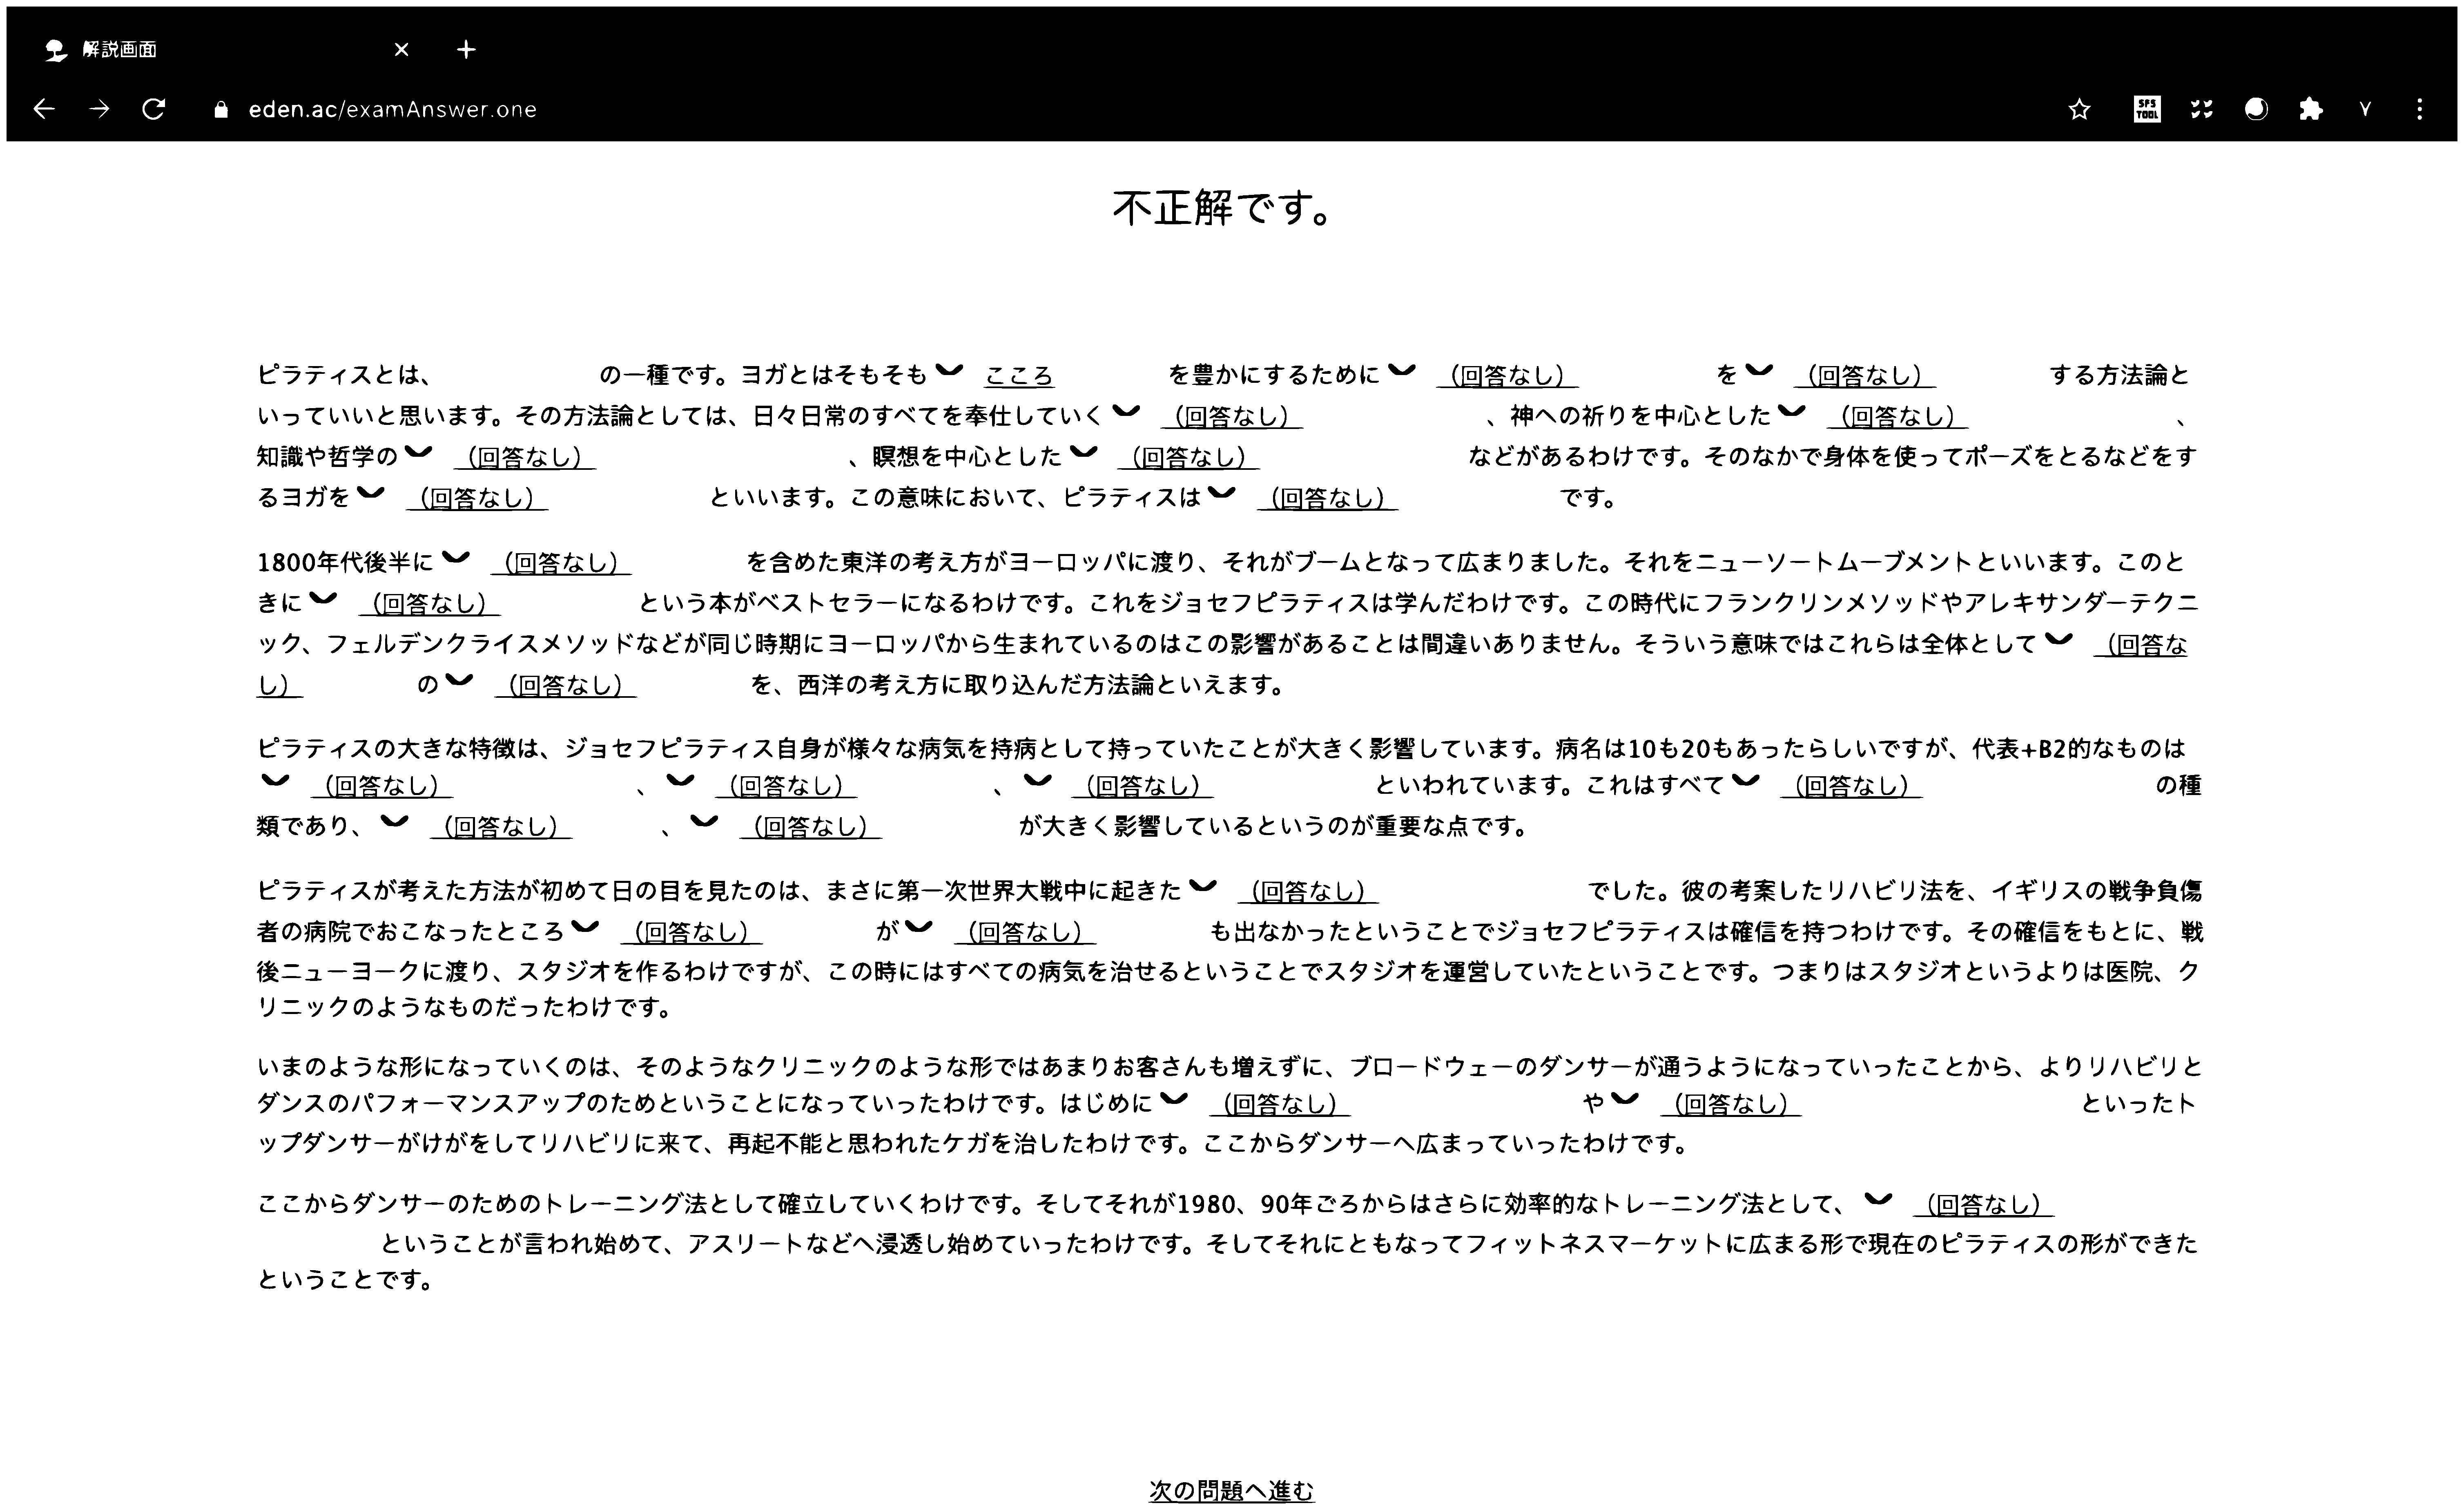
\includegraphics[scale=15cm]{img/hashrate.eps}
        \caption{2017年1月のハッシュレート分布 出典:Blockchain.info\cite{bitcoinhashrate}}
        \label{img:hashrate}
    \end{center}
\end{figure}
\fi

\if0
\begin{figure}[hbtp]
\includegraphics[width=15cm]{img/auzrk-ytelz.eps}
	\caption{活性化関数の歴史}
	\label{history_af}
\end{figure}
\fi
\chapter{本研究における問題定義と仮説}
\label{issue}

本章では、序章\ref{introduction}の内容及び背景\ref{background}の記述を踏まえて、本研究で取り組む課題とその解決要件を定義する。また、自身の仮説についても記述する。

\section{問題定義}
新型コロナウイルス感染拡大時のトイレットペーパーをめぐる流言と買いだめの発生について調査した『新型コロナウイルス感染拡大と流言・トイレットペーパー買いだめ〜報道のあり方を考える〜』~\cite{現状}の内容を参考に、現状のトイレットペーパー買いだめの状況・問題点を列挙し、整理する。

\subsection{新型コロナウイルス感染拡大時のトイレットペーパー買いだめ状況}

新型コロナウイルスの感染拡大に伴い、マスクなどの衛生用品だけでなく、生活必需品の買いだめが世界各地で起きている。
日本では2020年2月にトイレットペーパーの買いだめが発生して、全国に普及した。
各地のスーパーやドラックストア、コンビニにトイレットペーパーを買い求める人が殺到して、トイレットペーパーの品切れ状態となった。
そうした状況から、1人あたりの販売数量を制限する店舗も見られた。
買いだめの状況はその後、3月に入っても収まることはなく、入荷直後に売り切れてしまう状態が続いた。
ネット上で出品されたものの中には、通常の数倍以上の値段で取引されるものもあった。
トイレットペーパーのメーカー各社は連日24時間フル操業で生産を続けていた。
また、メーカーや卸売事業者・小売事業者が協力して店頭への配送を通常の倍に増やすなど、消費者の不安を解消するための努力が続けられた。
その結果、店頭での品薄状態は、地方では3月いっぱいでほぼ解消し、東京の都心部などでは4月中旬から下旬にかけてようやく収束に向かった。

\subsubsection{解決策の効果}

流言の打ち消しの効果\\*
実際に品切れの様子がテレビ等で報道された\\*
打ち消しするツイートは効果がなかった\\*
むしろ打ち消し情報と現実との違いに戸惑う人が増えて買いだめが加速した\\*

\subsubsection{本研究における問題定義}
予言の自己成就の概念のような、トイレットペーパーが不足するという根拠のない噂が現実になってしまうことを回避する必要がある。
実際に「トイレットペーパーが不足する」という根拠のない噂から、実際に各地のコンビニやスーパーやドラッグストアにトイレットペーパーを買い求める人びとが殺到し、店頭からトイレットペーパーが消えてしまった。
そうした問題について理解するためには、現象をコンピュータ上で再現することでそれらの構造を明らかにするべきである。
また、再現した現象に対して、問題の発生を防止するための施策を講じることが求められる。

\subsubsection{問題解決のための要件}
問題解決の要件として、1つは実社会におけるトイレットペーパー買いだめ問題の様相をシミュレーション上で正確に再現することである。
実社会で発生する問題の構造を理解するために、より正確なモデルを再現することが必要となる。
2つめは、施策の効果を検証することである。
問題の発生を防止するべく、より実社会において実現性の高い施策がどの程度効果を発揮するかを検証することが必要となる。

\subsubsection{仮説}
トイレットペーパー買いだめの様相を再現するにあたり、感染症の拡大におけるウイルスの拡散の様相を再現したシミュレーションを参考にすることができると考える。
買いだめが起きる際、まず「近いうちにトイレットペーパーが不足する」という誤った情報が拡散する。その誤情報の拡散がやがてトイレットペーパーの買いだめを引き起こすことになるが、そうした誤情報の拡散は感染症拡大におけるウイルスの拡散と同相であると考えることができる。
よって、感染症拡大のシミュレーションを参考にすることで、実社会におけるトイレットペーパー買いだめの様相を正確に再現することができる。

また、再現したシミュレーションの中で、各個人が誤った噂を広めることがないように噂の拡散に対して制限を設けること、あるいは問題に関わる個人全体に対して買いだめを自粛するように制限を設けるという対策を講じる。
以上の2つの対策により、買いだめの発生を防止して社会問題となるようなパニック状態を回避することができるのではないかと推測できる。

%%% Local Variables:
%%% mode: japanese-latex
%%% TeX-master: "./thesis"
%%% End:

\chapter{提案手法}
\label{proposed}

本章では提案手法について述べる.

(主に感染症シミュレーションが購買シミュレーションとどう呼応しているかについて)

\section{概要}

本研究では、感染症シミュレーションを参考にして購買シミュレーションを実行する。
感染症シミュレーションにおける「各エージェントの歩幅」、「エージェント同士の接触」、「感染症への感染」という定義はぞれぞれ購買シミュレーションにおいては、「各エージェントによる噂の伝播」、「買いだめの実状の目撃」、「買いだめ行為」と考えることができる。
また、感染症シミュレーションにおける人々の「免疫獲得」という状態は、購買シミュレーションにおいては「誤った情報を拡散しない状態」であり、そうした「免疫」の獲得を通して人々は正しい認識を得た状態であると見立てることができる。
これらを踏まえて、マルチエージェントシミュレーションを行い、実社会で起きたトイレットペーパー買いだめの様相をコンピュータ上で正確に再現する。
そして買いだめによる問題の発生を確認後、それらの問題の発生を防止するために「各エージェントによる噂の伝播」と「買いだめの実情の目撃」との2点に対して制限を設けることで対策を講じ、その効果を検証する。

\section{本実験で参考にする感染症シミュレーション(背景に入れるべきか?)}
本研究で参考にしている書籍『pythonによる数値計算とシミュレーション』~\cite{感染症}の中で扱われている感染症シミュレーションについて説明する。
感染症シミュレーションにあたり、まずプログラムにより仮想世界を構築し、その中でソフトウェア製のロボットであるエージェントを動かすことを行う。
シミュレーションの対象としては、2次元平面を移動する複数のエージェントを考える。
また、エージェントはそれぞれ内部状態を持っており、環境や他のエージェントと相互作用することができる。\\*

エージェントに対しては以下のような情報を与えている。

\begin{itemize}
  \item 空間内の座標
  \item 歩幅(移動速度)
  \item 状態(健康・感染・免疫獲得)
  \item 活動(移動)制限の有無(感染状態のエージェントに対して)
  \item 活動(移動)自粛の有無(すべてのエージェントに対して)
\end{itemize}

また、各エージェントの行動ルールは以下のように定められている。

\begin{itemize}
  \item 各エージェントは空間内のみを直線的に動き回り、空間の端に到達すると反射する。
  \item 「感染」状態及びそれに関するルールは以下とする。
  \begin{itemize}
    \item 「感染」状態のエージェントが「健康」のエージェントを中心とする一定範囲R(定数)に入った場合、「健康」エージェントは「感染」へと変化する。
    \item 「感染」エージェントが活動(移動)を制限された場合、活動(移動)範囲はR/4となる。
    \item 一定期間「感染」の状態が続くとそのエージェントは「免疫獲得」となり、「健康」エージェントを「感染」へと変化させる影響力を持たなくなる。
  \end{itemize}  
\end{itemize}

\section{本実験における設定}
本研究で扱う「トイレットペーパー買いだめ」のシミュレーション設計について説明する。

\subsection{各エージェントの属性}
実社会を表した空間を用意してエージェントをランダムに配置する。
その際、各エージェントには以下のような属性を与える。

\begin{itemize}
  \item 空間内の座標
  \item 噂の拡散力(他者への影響力)
  \item 状態(影響を受けやすい・買いだめ・合理的判断・思考停止)
  \item 噂の拡散に対する制限の有無(買いだめをするエージェントに対してのみ)
  \item 噂の拡散に対する自粛の有無(すべてのエージェントに対して)

\end{itemize}

\subsubsection{各エージェントの行動ルール}
各エージェントの行動のルールは以下のように定める。

\begin{itemize}
  \item 各エージェントは空間内のみを直線的に動き回り、空間の端に到達すると反射する。
  \item 状態が思考停止となったエージェントは他者に対する影響力を失い、座標が変化しないものとする。
  \item 買いだめ状態に関するルールは以下とする。
  \begin{itemize}
    \item 「影響を受けやすい」状態のエージェントが「買いだめ」のエージェントを中心とする一定範囲R(定数)に入った場合、「影響を受けやすい」エージェントは「買いだめ」を行う。
    \item 「買いだめ」エージェントが噂の拡散を制限された場合、拡散の範囲はR/4となる。
    \item 一定期間「買いだめ」の状態が続くとそのエージェントは誤情報に気付き「合理的判断」となる。
  \end{itemize}  
  \item 「買いだめ」エージェントは一定の確率で「思考停止」の状態となる。なお、「思考停止」の状態になりうるエージェントはエージェント生成時に決定している。
\end{itemize}

以上のルールのもとで、エージェントを空間内で自由に動き回らせ、「トイレットペーパーが不足する」という誤情報がどのように広がり、それに伴って買いだめ問題の発生状況を確認する。

\subsubsection{解決策の実行}
購買シミュレーションを実装して、実社会で起きるトイレットペーパー買いだめ問題の様相を再現した後、それらの問題の発生を防止するべく、解決策となる要素を入れ込み同シミュレーション上で実行する。
本研究において筆者が提案する解決策は以下の2点である。

\begin{itemize}
  \item 「買いだめ」状態のエージェントに対して、そのエージェントの噂の拡散力に対して制限を加える。
  \item すべてのエージェントに対して、噂の拡散を自粛するように制限を加える。
\end{itemize}

1つ目については、「買いだめ」状態のエージェントに対してのみ噂の拡散を行う。2つ目は、すべてのエージェントに対して噂の拡散に制限を設けることから、1つ目よりもより高い効果が得られると考える。
また、2つの対策を組み合わせて同時に実行することで、実社会でも適用可能性のある対策としてより高い効果が得られると推測する。


%%% Local Variables:
%%% mode: japanese-latex
%%% TeX-master: "../bthesis"
%%% End:

\chapter{実験}
\label{implementation}

本章では提案手法の実装について述べる.

\section{概要}

\section{プログラム構成}
図を入れて説明する

\subsection{グローバル変数の設定}
設定した数値の説明

実測値に基づいた数値設定である旨を書く

\subsection{Agentクラスの作成}

\subsection{シミュレーションの計算の定義}

\subsection{グラフの描画の設定}

\subsection{シミュレーションの実行}

\begin{lstlisting}[caption=hoge,label=fuga]
#include<stdio.h>
int main(){
   printf("Hello world!");
}
\end{lstlisting}


%%% Local Variables:
%%% mode: japanese-latex
%%% TeX-master: "../bthesis"
%%% End:

\chapter{評価}
\label{evaluation}
本章では,提案システムの評価について述べる.

\section{評価内容}

グラフを載せる\\*
結果(数値一覧)を一部載せる

\section{関連研究}



%%% Local Variables:
%%% mode: japanese-latex
%%% TeX-master: "./thesis"
%%% End:

\chapter{結論}
\label{conclusion}

本章では,本研究のまとめと今後の課題を示す.

\section{本研究のまとめ}

\section{本研究の課題}

%%% Local Variables:
%%% mode: japanese-latex
%%% TeX-master: "../thesis"
%%% End:

\appendix
\chapter{付録だよ}


\section{付録内容だよ}

書くよ

\chapter*{謝辞}
\addcontentsline{toc}{chapter}{謝辞}
\label{thanks}

謝辞を書きます。




%%% Local Variables:
%%% mode: japanese-latex
%%% TeX-master: "../yummy_bthesis"
%%% End:


\renewcommand{\thechapter}{\Alph{chapter}}
\setcounter{chapter}{0}
\vspace{-5mm}


\bibliographystyle{unsrt}\pagestyle{plain}
\bibliography{./bib/cites}\pagestyle{plain}
\thispagestyle{plain}%bibtex


\end{document}

%%% Local Variables:
%%% mode: japanese-latex
%%% TeX-master: t
%%% End:
